\chapter*{Results}
\label{chap:Results}
\setcounter{section}{0}

During my thesis i learnt a lot about posture and sensors and achieved a great base for further projects and continuing this journey. I definitely did not create a finished product, however this was never the goal of this projects. Non the less i achieved a view goals which I have listed below.

\section{Achieved Goals}

Transferring data
Simplyfied "sensor packets"
Improved reusability
Detecting posture
Visualsing posture


\section{Open Goals}

Usable product
User friendlyness
Self provisoning

\section{Similar Products}

SMING

\begin{wrapfigure}{R}{0.15\textwidth}
  \begin{center}
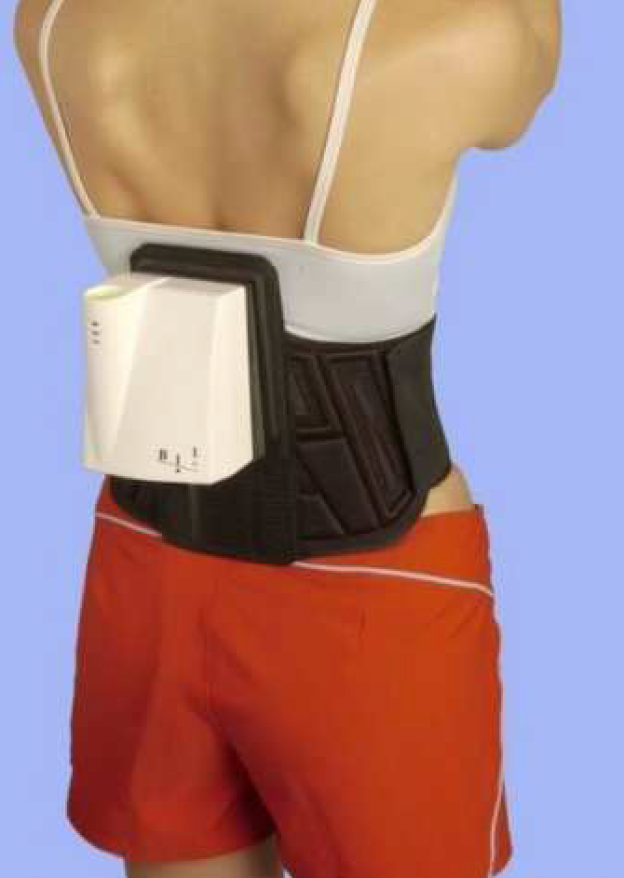
\includegraphics[width=\linewidth]{images/Swaystar_01.png}
  \end{center}
  \caption{\label{fig:swaystar}Swaystar}
\end{wrapfigure}
A Very important part of any "new" product is investigating what already exists on the market.
Usually someone already had a similar idea, or something which tries to solve the same problems has already been produced. 

In my case, an existing product was the trigger for my project idea. The so called swaystar \ref{fig:swaystar} offers almost the same functionality, however it is at least 10 times bigger and costs about 10'000 CHF. 
I have never used such a device, however i have talked to people who worked with one. Apparently it tracks the movement / positioning of users and stores the data. An additional headband can be purchased with which vibrations are sent to the user so he can improve his body ergonomics and balance. 

As said, it offers a very similar functionality, however not it covers the same use cases. Due to the size and price it can almost exclusively only be used in therapies and by medical professionals. My device intends to target the end user, and offer an easier and more affordable solution. The swaystar also is closed-source and appears to be a rather old product.


\newpage

\begin{wrapfigure}{R}{0.3\textwidth}
  \begin{center}
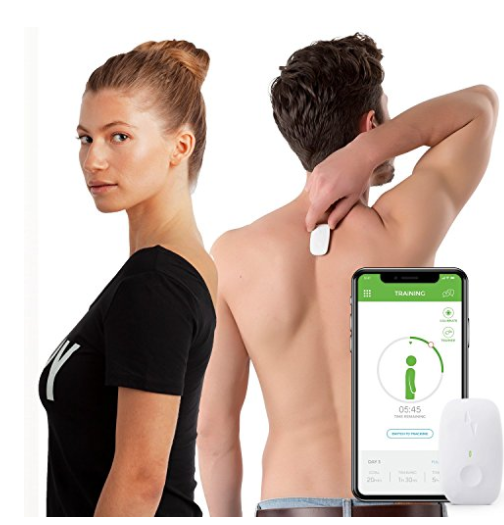
\includegraphics[width=0.3\textwidth]{images/Screenshot_3.png}
  \end{center}
  \caption{Go Posture trainer}
  \label{fig:gotrainer}
\end{wrapfigure}

Further investigations into other products, were almost fruitless. There are some apps which offer almost the same thing I have tried to achieve with my app, but a bit more refined and there is one product which offers a use-case that could be considered equal to the first defined use-case (improved sitting posture), at least on first glance (\ref{fig:gotrainer} Go Trainer). 

The product functions as a posture trainer, however it has to be attached to the back, and it is, even if small, quite visible under a shirt. Secondly the device only offers a mono-directional biofeedback. \cite{HowToImp2:online}

Furthermore the device is closed source and is only targeted to users who want to improve their posture. As mentioned the plan for my device would be to keep everything open-source and cover a wider range of use-cases. 

Most other devices to improve posture use cloth to physically "pull" the user in the right position.

After all these investigations and also further investigations into the medical field I considered my device to still be an innovation, offering something which is not yet available on the market.

\section{Learnings}

Amount of sensors needed
Positioning of sensor for useful posture
What is posture